\documentclass{article}\usepackage[]{graphicx}\usepackage[]{xcolor}
% maxwidth is the original width if it is less than linewidth
% otherwise use linewidth (to make sure the graphics do not exceed the margin)
\makeatletter
\def\maxwidth{ %
  \ifdim\Gin@nat@width>\linewidth
    \linewidth
  \else
    \Gin@nat@width
  \fi
}
\makeatother

\definecolor{fgcolor}{rgb}{0.345, 0.345, 0.345}
\newcommand{\hlnum}[1]{\textcolor[rgb]{0.686,0.059,0.569}{#1}}%
\newcommand{\hlstr}[1]{\textcolor[rgb]{0.192,0.494,0.8}{#1}}%
\newcommand{\hlcom}[1]{\textcolor[rgb]{0.678,0.584,0.686}{\textit{#1}}}%
\newcommand{\hlopt}[1]{\textcolor[rgb]{0,0,0}{#1}}%
\newcommand{\hlstd}[1]{\textcolor[rgb]{0.345,0.345,0.345}{#1}}%
\newcommand{\hlkwa}[1]{\textcolor[rgb]{0.161,0.373,0.58}{\textbf{#1}}}%
\newcommand{\hlkwb}[1]{\textcolor[rgb]{0.69,0.353,0.396}{#1}}%
\newcommand{\hlkwc}[1]{\textcolor[rgb]{0.333,0.667,0.333}{#1}}%
\newcommand{\hlkwd}[1]{\textcolor[rgb]{0.737,0.353,0.396}{\textbf{#1}}}%
\let\hlipl\hlkwb

\usepackage{framed}
\makeatletter
\newenvironment{kframe}{%
 \def\at@end@of@kframe{}%
 \ifinner\ifhmode%
  \def\at@end@of@kframe{\end{minipage}}%
  \begin{minipage}{\columnwidth}%
 \fi\fi%
 \def\FrameCommand##1{\hskip\@totalleftmargin \hskip-\fboxsep
 \colorbox{shadecolor}{##1}\hskip-\fboxsep
     % There is no \\@totalrightmargin, so:
     \hskip-\linewidth \hskip-\@totalleftmargin \hskip\columnwidth}%
 \MakeFramed {\advance\hsize-\width
   \@totalleftmargin\z@ \linewidth\hsize
   \@setminipage}}%
 {\par\unskip\endMakeFramed%
 \at@end@of@kframe}
\makeatother

\definecolor{shadecolor}{rgb}{.97, .97, .97}
\definecolor{messagecolor}{rgb}{0, 0, 0}
\definecolor{warningcolor}{rgb}{1, 0, 1}
\definecolor{errorcolor}{rgb}{1, 0, 0}
\newenvironment{knitrout}{}{} % an empty environment to be redefined in TeX

\usepackage{alltt}
\usepackage{graphicx}
\usepackage[top=.5in,bottom=.5in,right=1in,left=1in]{geometry}% http://ctan.org/pkg/geometry

\usepackage[colorlinks = true,
            linkcolor = blue,
            urlcolor  = blue,
            citecolor = blue,
            anchorcolor = blue]{hyperref}
            
\setcounter{secnumdepth}{1}
\setcounter{tocdepth}{1}

\newenvironment{itemize*}%
  {\begin{itemize}%
    \setlength{\itemsep}{0pt}%
    \setlength{\parskip}{0pt}}%
  {\end{itemize}}
	
\newenvironment{enumerate*}%
  {\begin{enumerate}%
    \setlength{\itemsep}{0pt}%
    \setlength{\parskip}{0pt}}%
  {\end{enumerate}}
  
\renewcommand\labelitemi{$\vcenter{\hbox{\tiny$\bullet$}}$}

\setcounter{secnumdepth}{0}

\title{Environmental Analysis Course Plans}
\date{\today}
%\author{}
\IfFileExists{upquote.sty}{\usepackage{upquote}}{}
\begin{document}

\begin{titlepage}
\thispagestyle{empty}

\begin{figure}%{}{-10cm}
\includegraphics[width=1.0\textwidth]{"/home/mwl04747/beginnersluck/docs/figures/Exhibition"}
\caption{From the Anthropocene exhibition at the Art Gallery of Ontario – AGO in Toronto.}
\end{figure}


\maketitle
\tableofcontents

\end{titlepage}

\newgeometry{top=1in,bottom=1in,right=1.5in,left=1.5in}



\newpage
\section{Sustainable Built Environment}



\subsection{Faculty Advsisor(s)}

\begin{itemize*}
  \item Char Miller (Professor of Environmental Analysis)
\end{itemize*}

\subsection{Affiliated Faculty}

\begin{itemize*}
  \item Lance Neckar (Professor of Environmental Analysis -- Pitzer)
  \item George Gorse (Professor of Art History)
  \item Albert Park (Professor of History -- CMC)
%  \item advisors.sbe$Affiliated4
\end{itemize*}

\subsection{Description}

The Sustainability and the Built Environment Concentration (SBE) focuses on urban planning, design and architecture. 

The SBE course plan interrogates the built environment, whether urban, suburban, or rural (and every place in between). It is designed for students seeking a comprehensive curriculum that is focused on how to plan, design, construct and manage communities from a more sustainable perspective. Learn about the latest planning approaches and policy/regulatory requirement; green architecture, sustainable site design and landscapes; renewable energy and energy efficiency; sustainable water resources management; and green infrastructure. Acquire the skills necessary to integrate sustainable design principles into long-range visions and the day-to-day development and management of the built environment.


\subsection{Course Requirements (12 Courses)}

\begin{description}

  \item[Core Courses] Complete all three of these following:
  
\begin{itemize*}
  \item EA010~--~Introduction to Environmental Analysis~(every semester)
  \item EA020~--~Society, Culture and Environment~(every semester)
  \item EA030~--~Science and the Environment~(every semester)
\end{itemize*}

  \item[Senior Exercise] Complete one of the following:
  
\begin{itemize*}
  \item EA190 PO~--~Senior Clinic~(every spring)
  \item EA191 PO~--~Senior Thesis~(every fall)
\end{itemize*}


\item[Design and Representation] Complete at least one design and representation course. For example, ART005 PO, ART010 PO, ART020 PO, ART021 PO, ART101 SC, ART105 SC, ART120 SC, ART121 SC, ART125 SC, EA101 PO.



\item[Design Studio/Labs] Complete at least one design studio course or lab. Examples might include: EA133 PZ, EA134 PZ, EA185 PO.



\item[Electives] Elective courses in SBE should be selected in close consultation with the major adviser and coordinator. Select five courses from the following or similar options, generally no more than two from a group:
\begin{itemize}
  \item Urban history, geography, theory and ecology
  \item Design and Planning
  \item Environmental Justice/Policy/Economics/Sociology
\end{itemize}

\noindent Electives might include: ANTH113 SC, ANTH144 PO, ARHI188 SC, ARHS179 PO, EA130 PZ, BIOL104 PO, BIOL104 PO, BIOL108 PO, EA085 PO, EA106 PZ, EA171 PO, EA172 PO, EA173 PO, EA180 PO, EA189F PO, EA189M PO, GEOG 179 HM, PHIL037 PO, POLI060 PO, POLI061 PO.



\end{description}


\newpage %#######################################################################
\section{Race, Class, and Gender}



\subsection{Faculty Advsisor(s)}

\begin{itemize*}
  \item Aimee Bahng (Associate Professor of Gender and Women Studies)
\end{itemize*}

\subsection{Affiliated Faculty}

\begin{itemize*}
  \item Erin Runions (Professor of Religious Studies)
  \item TBD (Scripps)
  \item TBD (Scripps)
\end{itemize*}

\subsection{Description}

The Race, Class, and Gender course plan explores the implications of race, class, and gender on environmental problem-solving and decision making. Students apply theory and approaches in analyzing race, class, and gender to clarify and respond to environmental issues. Students will critically evaluate, synthesize, and analyze environmental issues using the scholarly literature on the intersection of race, class and gender constructions and how these define access to resources and exposure to hazards.

\subsection{Course Requirements (12 Courses)}

\begin{description}
  
 \item[Core Courses] Complete all three of these following:
  
\begin{itemize*}
  \item EA010~--~Introduction to Environmental Analysis~(every semester)
  \item EA020~--~Society, Culture and Environment~(every semester)
  \item EA030~--~Science and the Environment~(every semester)
\end{itemize*}

  \item[Senior Exercise] Complete one of the following:
  
\begin{itemize*}
  \item EA190 PO~--~Senior Clinic~(every spring)
  \item EA191 PO~--~Senior Thesis~(every fall)
\end{itemize*}


  \item[Environmental Justice] Select one of the following courses:
  
% latex table generated in R 4.2.1 by xtable 1.8-4 package
% Thu Nov 14 14:42:35 2024
\begin{table}[ht]
\centering
\begin{tabular}{lll}
  \hline
CourseNo & Title & Offered \\ 
  \hline
ANTH144 PO & Anthropology of Environmental Justice & irregularly \\ 
  EA086 & Environmental Justice & Spring 2025 \\ 
  EA099 PO & Urban Health Equity & irregularly \\ 
  GWS172 PO & Race, Gender \& Environment & every spring \\ 
   \hline
\end{tabular}
\end{table}


  \item[Area and Ethnic?? Studies] Select three courses from one of the Area Studies or Studies, one of which must be an introductory, and two of which must in be in the same program or department. Two courses can overlap between categories where intersectionality is a central component of the course.
  
\begin{itemize*}
  \item Chincanx-Latinx Studies (\href{https://catalog.pomona.edu/preview_entity.php?catoid=47&ent_oid=2387}{Intercollegiate Course Catalog})
  \item Asian American Studies (\href{https://catalog.pomona.edu/preview_entity.php?catoid=47&ent_oid=2381}{5C Asian American Course Catalog})
  \item Asian Studies (\href{https://catalog.pomona.edu/preview_entity.php?catoid=47&ent_oid=2383}{5C Asian Studies Course Catalog})
  \item Africana Studies (\href{https://colleges.claremont.edu/africana-studies/}{Intercollegiate Department of Africana Studies})
  \item Russian and Eastern European Studies (\href{https://www.pomona.edu/academics/departments/russian/courses-requirements/rees}{Current Russian and REES Courses})
  \item Middle Eastern Studies (\href{https://catalog.pomona.edu/preview_entity.php?catoid=47&ent_oid=2383}{5C Middle-East Studies Course Catalog})
  \item German Studies (\ref{https://www.pomona.edu/academics/majors/german-studies}{German Studies Major})
  \item Latin American Studies (\ref{https://www.pomona.edu/academics/majors/latin-american-studies}{Latin American Studies Major})
\end{itemize*}

  
  \item[Class] Select three courses that focus on class (by agreement with the advisor), e.g. Labor History, Economics of Economics, Globalization, and Colonization. The courses below might be examples: 
  
% latex table generated in R 4.2.1 by xtable 1.8-4 package
% Thu Nov 14 14:42:35 2024
\begin{table}[ht]
\centering
\begin{tabular}{lll}
  \hline
CourseNo & Title & Offered \\ 
  \hline
ECON122 PO & Poverty and Income Distribution & Spring, alternate years \\ 
  GEOG175 HM & Geographies of Labor & TBD \\ 
   \hline
\end{tabular}
\end{table}

  
  
  \item[Gender] Select three courses in Gender Studies:
  
% latex table generated in R 4.2.1 by xtable 1.8-4 package
% Thu Nov 14 14:42:35 2024
\begin{table}[ht]
\centering
\begin{tabular}{lll}
  \hline
CourseNo & Title & Offered \\ 
  \hline
EA162 PZ & Gender, Environment \& Development & TBD \\ 
  GWS026 PO & Introduction to Gender Studies & every semester \\ 
  GWS180 PO & Queer and Feminist Theories & last offered fall 2019 \\ 
  HIST101V PO & Gender, Sexuality and Feminisms in Modern East Asia & Last offered Fall 2017 \\ 
   \hline
\end{tabular}
\end{table}


\end{description}


\newpage
\section{Environmental Analysis---Economics}



\subsection{Faculty Advsisor(s)}

\begin{itemize*}
  \item Bowman Cutter (Associate Professor of Economics)
\end{itemize*}

\subsection{Affiliated Faculty}

\begin{itemize*}
  \item TBD (Scripps)
%  \item advisors.econ$Affiliated2
%  \item advisors.econ$Affiliated3
\end{itemize*}

\subsection{Description}

The most important questions concerning the environment often concern the interactions between production, consumption, and the environment.  Economics provides the analytical and computational tools to understand how economic and policy decisions affect the environment and in turn how the environment affects the economy.  Students in EA-Econ often go on to careers in energy, environmental consulting, urban planning, and other careers that require an understanding of the linkages between economics, the environment, and human well-being.

\subsection{Course Requirements (12 Courses)}

\begin{description}

  \item[Core Courses] Complete all three of these following:
  
\begin{itemize*}
  \item EA010~--~Introduction to Environmental Analysis~(every semester)
  \item EA020~--~Society, Culture and Environment~(every semester)
  \item EA030~--~Science and the Environment~(every semester)
\end{itemize*}

  \item[Senior Exercise] Complete one of the following:
  
\begin{itemize*}
  \item EA190 PO~--~Senior Clinic~(every spring)
  \item EA191 PO~--~Senior Thesis~(every fall)
\end{itemize*}



\item[Foundations of Economics] EA-Econ students will take the following 4 courses to provide a basic background knowledge with the following courses:


\begin{itemize*}
  \item ECON051~--~Introduction to Macroeconomics~(every semester)
  \item ECON052~--~Introduction to Microeconomics~(every semester)
  \item ECON057 PO~--~Economics Statistics~(every semester)
  \item ECON102 PO~--~Microeconomic Theory~(every semester)
\end{itemize*}

\item[Environmental Applications] to build content specialization, EA-Econ students will take two of the following 4 courses:

\begin{itemize*}
  \item ECON124 PO~--~Water Resource Economics and Management~(irregularly)
  \item ECON125 PO~--~Natural Resource Economics and Policy~(Spring 2025)
  \item ECON127 PO~--~Environmental Economics~(every fall)
%  \item econ.apps$Course[4]
\end{itemize*}

\item[Methods] EA-Econ students must take atleast one methods course prior to the senior capstone course:

\begin{itemize*}
  \item ECON107 PO~--~Applied Econometrics~(every semester)
  \item ECON150+ PO~--~Other higher-level course~(every semester)
%  \item econ.methods$Course[3]
%  \item econ.methods$Course[4]
\end{itemize*}

\item[Electives] One of the courses or an acceptable substitute from each of the following two categories to provide additional insight into the field:

\noindent \textbf{Public Policy Analysis and Politics} (Potential Available Courses = 8)

\begin{itemize*}
  \item EA189M PO~--~Desert Conservation Field Seminar~(irregularly)
  \item POLI039 PO~--~Politics of Environmental Justice~(delisted)
  \item POLI060 PO~--~Global Politics of Food and Agriculture~(every spring)
  \item POLI061 PO~--~Global Politics of Water~(Fall 2023)
  \item POST115 HM~--~Comparative Environmental Politics~(TBD)
  \item POST140 HM~--~Global Environmental Politics~(Fall 2024)
  \item PPA001 PO~--~Introduction to Public Policy Analysis~(every fall)
  \item SOSC180 HM~--~Tropical Forests: Policy and Practice~(TBD)
%  \item econ.PPA$Course[9]
%  \item econ.PPA$Course[10]
\end{itemize*}

%\noindent Anthropology \& History (n = nrow(econ.anthro))

%\begin{itemize*}
%  \item econ.anthro$Course[1]
%  \item econ.anthro$Course[2]
  %\item econ.anthro$Course[3]
%\end{itemize*}

%\noindent Values and Ethics (n = nrow(econ.values))

%\begin{itemize*}
%  \item econ.values$Course[1]
%\end{itemize*}
  
\noindent\textbf{ Natural Sciences} (Potential Courses Available = 5)\footnote{higher level environmental related science courses with pre-requisites are likely to be approved; please clear with advisor}

\begin{itemize*}
  \item CHEM112 PO~--~Analysis of Scientific Literature~(delisted)
  \item EA085 PO~--~Food, Land, and Environment~(Spring 2029)
  \item EA103 NS~--~Soils and the Environment~(Spring 2025)
  \item GEOL 20C PO~--~Environmental Geology~(Spring 2025)
  \item GEOL20G PO~--~Climate Change~(Fall 2024)
%  \item econ.methods$Course[4]
\end{itemize*}

\end{description}



\begin{figure}
\centering
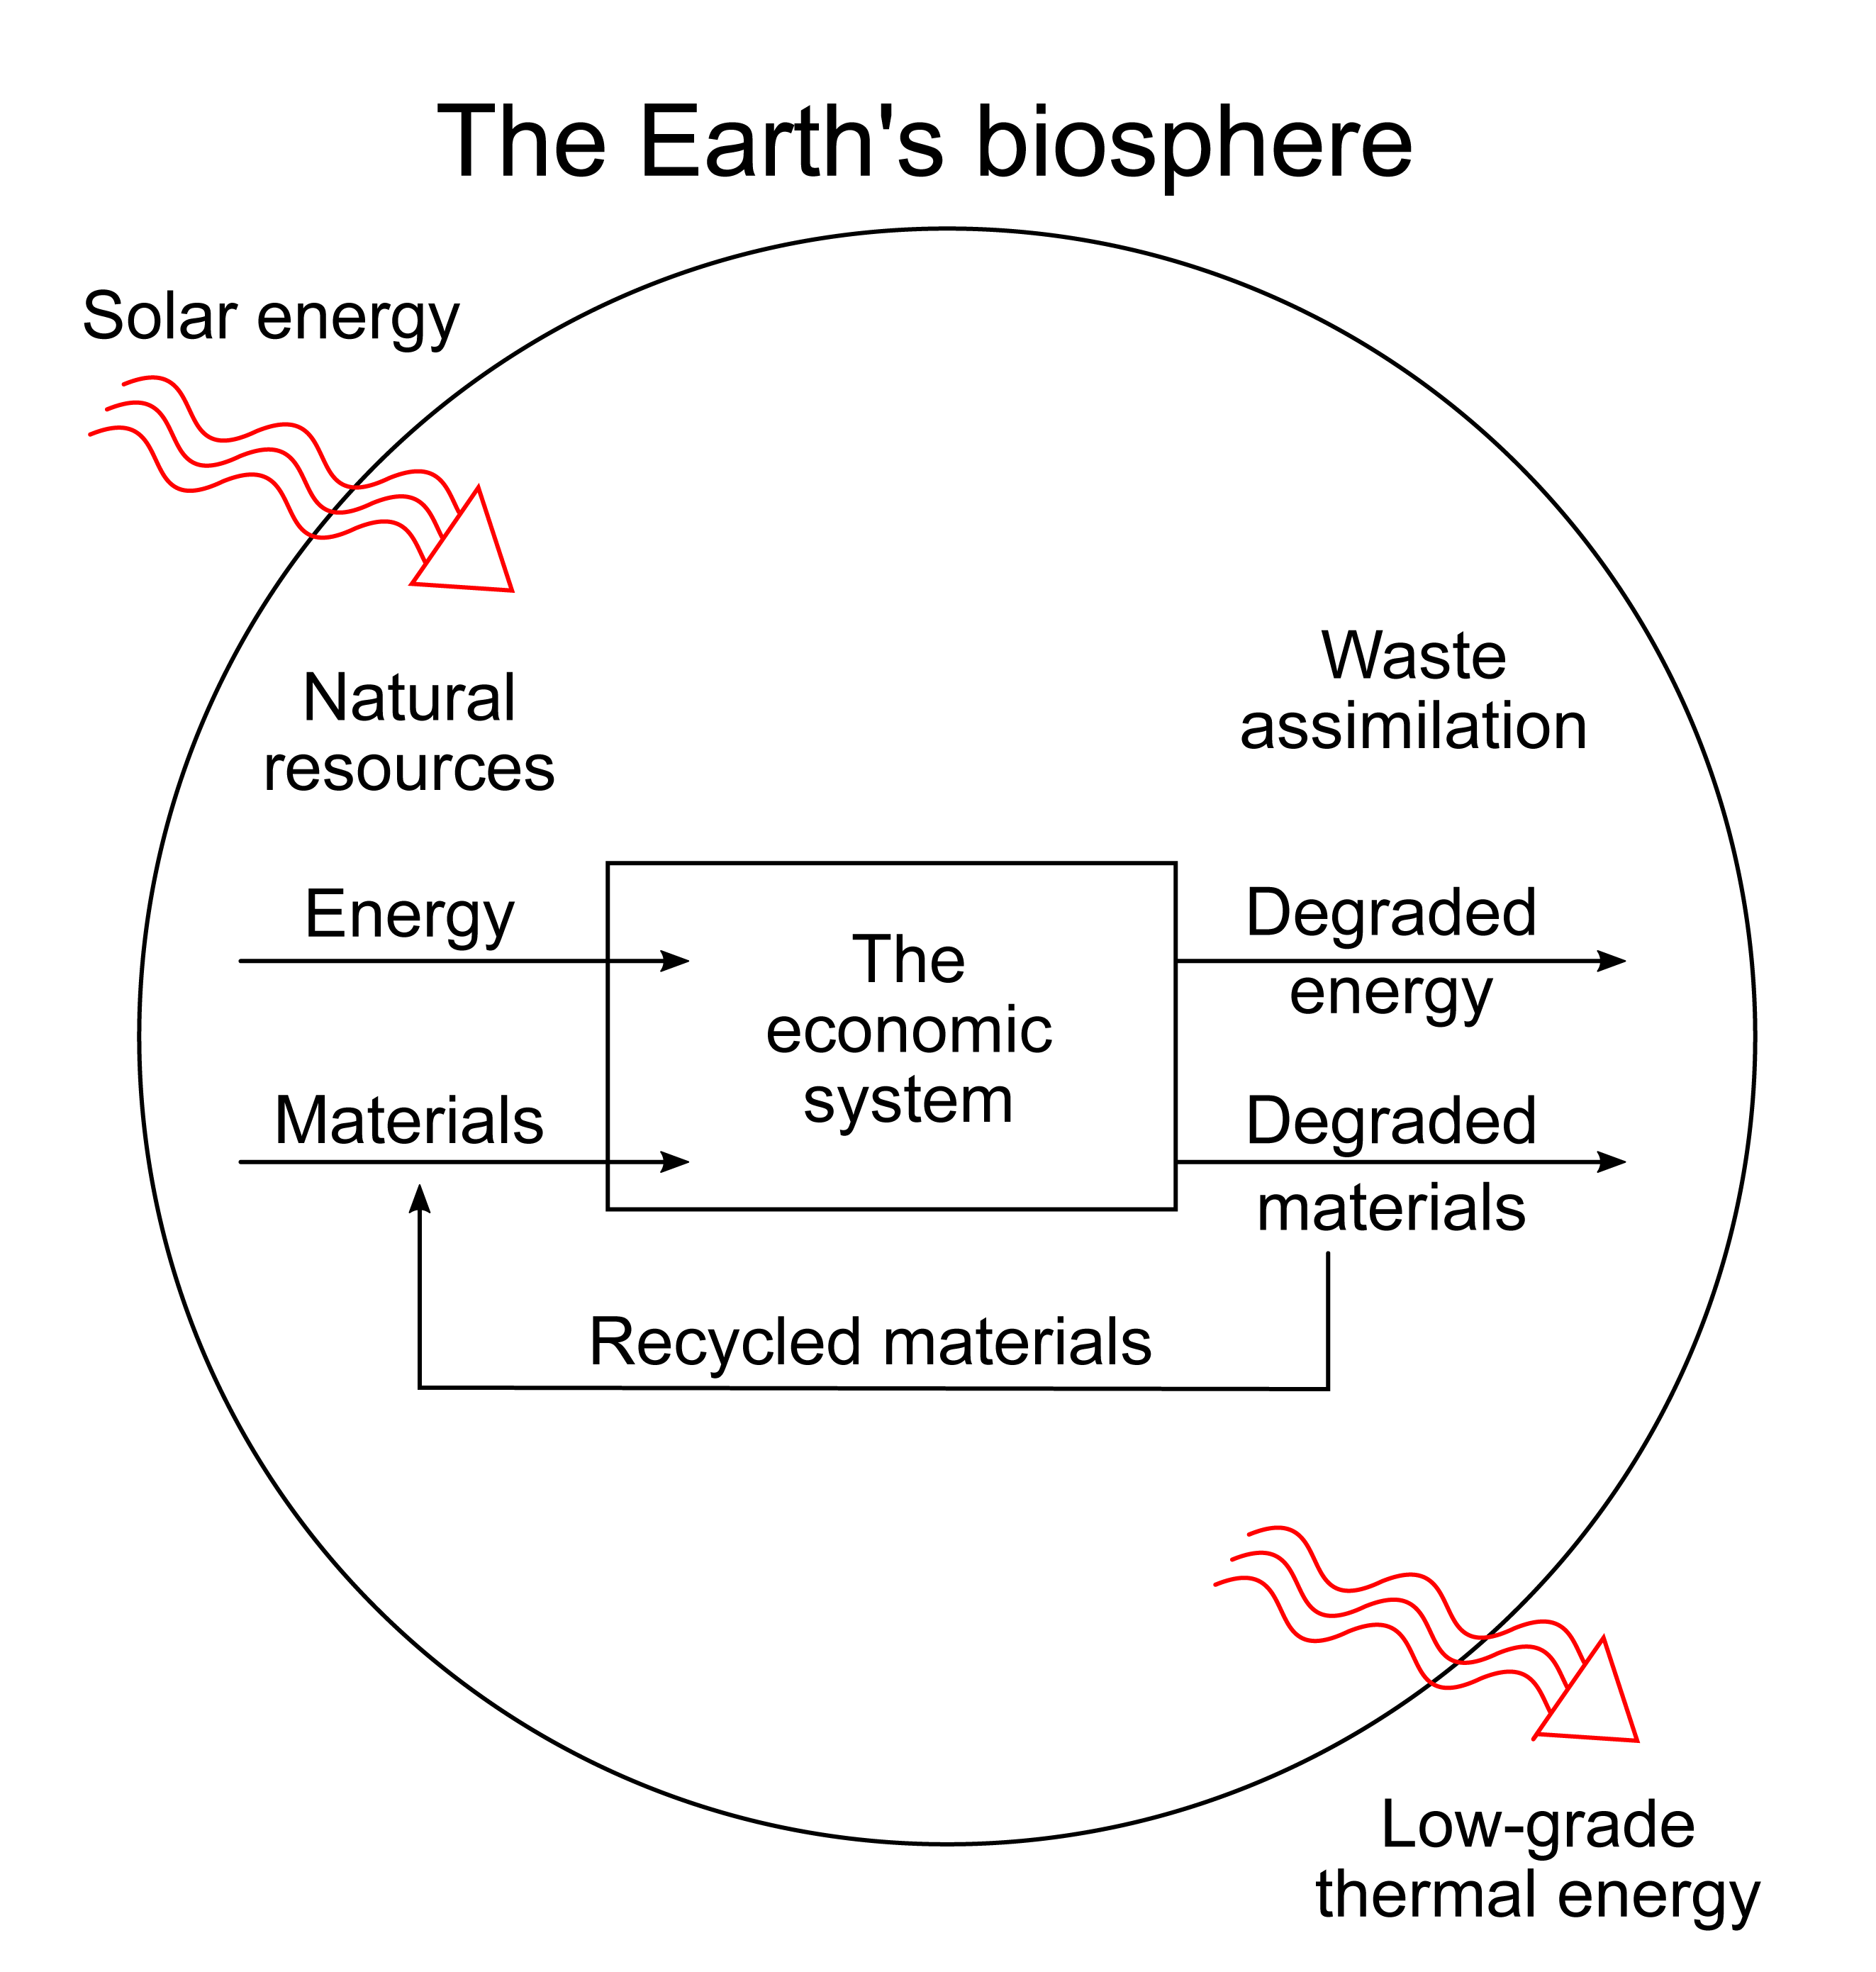
\includegraphics[width=0.60\textwidth]{/home/mwl04747/beginnersluck/docs/figures/Diagram_of_natural_resource_flows-en.png}
\caption{Diagram describing the flow of natural resources through the economy: Valuable resources are procured from nature by the input end of the economy; the resources flow through the economy, being transformed and manufactured into goods along the way; and invaluable waste and pollution eventually accumulate by the output end. Recycling of material resources is possible, but only by using up some energy resources as well as an additional amount of other material resources; and energy resources, in turn, cannot be recycled at all, but are dissipated as waste heat.}
\end{figure}


\newpage %######################################################################################
\section{Environmental Geology}



\subsection{Faculty Advsisor(s)}

\begin{itemize*}
  \item Jade Star Lackey (Professor of Geology)
\end{itemize*}

\subsection{Affiliated Faculty}

\begin{itemize*}
  \item Colin Robbins (Associate Professor of Environmental Analsysis -- Natural Sciences Department)
  \item Bob Gaines (Professor of Geology)
  \item Eric Grofils (Professor of Geology)
\end{itemize*}

\subsection{Description}

The Geology and the Environment concentration is designed for students interested in the interaction of humans with Earth’s geology and physical systems.

\subsection{Course Requirements (12 Courses)}

\begin{description}

 \item[Core Courses] Complete all three of these following:
  
\begin{itemize*}
  \item EA010~--~Introduction to Environmental Analysis~(every semester)
  \item EA020~--~Society, Culture and Environment~(every semester)
  \item EA030~--~Science and the Environment~(every semester)
\end{itemize*}

  \item[Senior Exercise] Complete one of the following:
  
\begin{itemize*}
  \item EA190 PO~--~Senior Clinic~(every spring)
  \item EA191 PO~--~Senior Thesis~(every fall)
\end{itemize*}

\item[Geologic Introductions] Take one of the following courses: GEOL020A PO, GEOL020B PO, GEOL020C PO, GEOL020D PO, GEOL020G PO. 
  

\item[Geographic Information Systems] Take one of the following courses:

\begin{itemize*}
  \item EA101 PO~--~Just GIS!~(Spring 2025)
  \item GEOL189G PO~--~Introduction to GIS for Geologists~(Spring 2025)
\end{itemize*}

\item[Geologic Foundations] Take four of the foundation courses in Geology from ) potential courses:

\begin{itemize*}
  \item EA055L NS~--~Phys Geography and Geomorphology~(TBD)
  \item EA103 NS~--~Soils and the Environment~(Spring 2025)
  \item GEOL112 PO~--~Remote Sensing~(delisted)
  \item GEOL120 PO~--~Introduction to Geochemistry~(Maybe 2026)
  \item GEOL125 PO~--~Earth History~(Spring 2025)
\end{itemize*}

\item[Geological Interfaces] Take two courses from one of the following categories courses:

\textbf{Chemical Interfaces:} Take two introductory chemistry sources:

\begin{itemize*}
  \item CHEM001A PO~--~General Chemistry~(every fall)
  \item CHEM001B PO~--~General Chemistry~(every spring)
  \item CHEM051 PO~--~General Chemistry -- Accelerated~(Fall 2026)
  \item CHEM023A~--~General Chemistry Applications I~(Fall 2025)
  \item CHEM023B~--~General Chemistry Applications II~(Spring 2026)
\end{itemize*}

\textbf{Biological Interfaces:} Take two biology\footnote{most have prerequisites} from 11 potential courses: 

\begin{itemize*}
  \item BIOL040 PO~--~Introduction of Genetics~(every fall)
  \item BIOL041E PO~--~Introductory Ecology and Evolutionary Biology~(every spring)
  \item BIOL104 PO~--~Conservation Science~(every spring)
  \item BIOL104 PO~--~Fire Ecology~(irregularly)
  \item BIOL106 PO~--~Aquatic Ecology~(Fall 2024)
  \item BIOL107 PO~--~Invasion Biology~(Last offered Spring 2024)
  \item BIOL108 PO~--~Data Science of Conservation~(Spring 2025)
  \item BIOL116 PO~--~Ecology and Evolution of Plants~(Last offered Spring 2023)
  \item BIOL121 PO~--~Insect Ecology and Behavior~(Fall 2024)
  \item BIOL180 PO~--~Microbial Ecology~(Spring 2025)
\end{itemize*}

\textbf{Historical Interfaces:} Take from the following list of courses: 

\begin{itemize*}
  \item HIST068 CM~--~Disasters in the Ancient Mediterranean~(TBD)
  \item HIST096 CM~--~The Amazon~(TBD)
  \item HIST101A PO~--~Indian Ocean World~(last offered spring 2020)
  \item HIST101AC PO~--~Dark Ecologies~(fall alternate years)
  \item HIST101E PO~--~Science and Empire~(Last offered fall 2023)
  \item HIST186 PO~--~Climate in History~(Spring 2025)
  \item HIST113 CM~--~US Environmental History~(Spring 2025)
  \item HIST118??~--~Native American History~(Last offered spring 2023)
  \item HIST120 CM~--~History of the American West~(NA)
  \item HIST158 PZ~--~Ecological History~(TBD)
\end{itemize*}

\end{description}

\begin{figure}
\centering
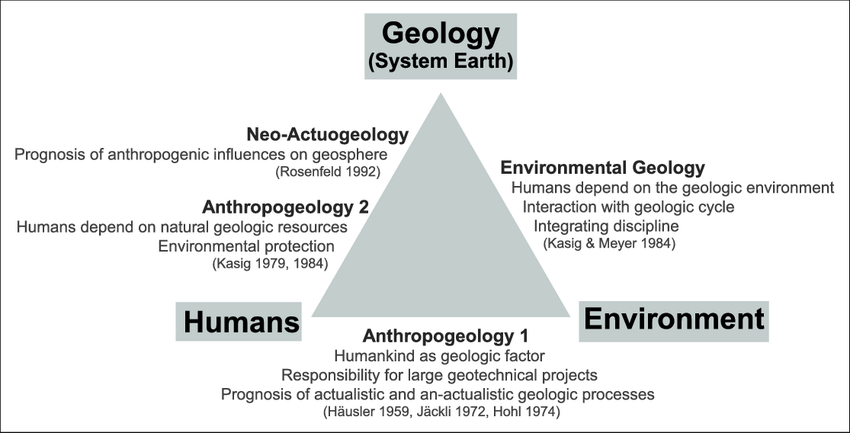
\includegraphics[width=0.60\textwidth]{/home/mwl04747/beginnersluck/docs/figures/Graphic-illustration-of-the-two-different-concepts-of-anthropogeology-of-environmental.png}
\caption{Graphic illustration of the two different concepts of anthropogeology, of environmental geology and neo-actuogeology in the context between geology, humans and environment (modified from Häusler Jr, 2016).}
\end{figure}

\newpage %##########################################################
\section{Environmental Biology}



\subsection{Faculty Advsisor(s)}

\begin{itemize*}
  \item Fran Hanzawa (Associate Professor of Biology)
\end{itemize*}

\subsection{Affiliated Faculty}

\begin{itemize*}
  \item Charlotte Chang (Assistant Professor of Biology and Environmental Analysis)
  \item Nina Karnovsky (Professor of Biology)
  \item Wallace "Marty" Meyer (Associate Professoer of Biology)
\end{itemize*}

\subsection{Description}

In the EA Biology course plan, students will focus their Environmental Analysis major by incorporating the biological sciences into their training, and focusing on methods of biological inquiry and understanding biological concepts.

Only one of the upper division Biology courses can be satisfied with a course from a study abroad program or domestic program. Pomona students may take courses that count towards the major at the other 5Cs if it is not offered at Pomona College.\footnote{Can be waived by advisor.} 

Many upper division biology courses have Biology 41C PO Intro Cell Chemistry and Cell Biology w/lab as a prerequisite. In addition, the EA-Biology faculty also strongly recommend taking organic chemistry (CHEM 110A and 110B), mathematics and statistics (MATH 31 or MATH 60 and MATH 58 or MATH 58B). 

Students interested in public policy might consider PPA-EA or PPA-Biology. 

\subsection{Course Requirements (12 Courses)}

\begin{description}

 \item[Core Courses] Complete all three of these following:
  
\begin{itemize*}
  \item EA010~--~Introduction to Environmental Analysis~(every semester)
  \item EA020~--~Society, Culture and Environment~(every semester)
  \item EA030~--~Science and the Environment~(every semester)
\end{itemize*}

  \item[Senior Exercise] Complete one of the following:
  
\begin{itemize*}
  \item EA190 PO~--~Senior Clinic~(every spring)
  \item EA191 PO~--~Senior Thesis~(every fall)
\end{itemize*}

%and ECON 52, Microeconomics. 


\item[Foundations in Biology] The following course are required.

\begin{itemize*}
  \item BIOL040 PO~--~Introduction of Genetics~(every fall)
  \item BIOL041E PO~--~Introductory Ecology and Evolutionary Biology~(every spring)
  \item CHEM001A PO~--~General Chemistry~(every fall)
  \item CHEM001B PO~--~General Chemistry~(every spring)
\end{itemize*}

\noindent CHEM051 substitute for CHEM001A and CHEM001B. 

  \item[Biology Lab-based courses] Student will take 2 of the 13 following courses: 

\begin{itemize*}
  \item BIOL104 PO~--~Conservation Science~(every spring)
  \item BIOL106 PO~--~Aquatic Ecology~(Fall 2024)
  \item BIOL107 PO~--~Invasion Biology~(Last offered Spring 2024)
  \item BIOL108 PO~--~Data Science of Conservation~(Spring 2025)
  \item BIOL112 PO~--~Advanced Animal Ecology~(Last offered Spring 2024)
  \item BIOL116 PO~--~Ecology and Evolution of Plants~(Last offered Spring 2023)
  \item BIOL125 PO~--~Animal Behavior~(Alt years - next Fall 2025)
  \item BIOL132 PO~--~Vertebrate Biology~(Last offered Fall 2022)
  \item BIOL140 PO~--~Animal Physiology~(Every  Fall)
  \item BIOL166 PO~--~Plant Physiology~(Last  offered Fall 2023)
  \item BIOL169 PO~--~Developmental Biology~(Every Spring)
  \item BIOL180 PO~--~Microbial Ecology~(Spring 2025)
  \item BIOL181 PO~--~Fire Ecology~(Last offered Spring 2015)
%  \item biol.lab$Course[2]
%  \item biol.lab$Course[3]
%  \item biol.lab$Course[4]
\end{itemize*}

\item[Seminar and Geology Options] Students will take an additional biology lab course or one of the following courses:

\begin{itemize*}
  \item BIOL104 PO~--~Fire Ecology~(irregularly)
%  \item biol.sem$Course[2]
  \item GEOL 20C PO~--~Environmental Geology~(Spring 2025)
  \item GEOL20G PO~--~Climate Change~(Fall 2024)
\end{itemize*}

\item[Social Sciences] EA-Biology students should also take an applicable social sciece course with consultation with their advisor. Below are potential options: 

% latex table generated in R 4.2.1 by xtable 1.8-4 package
% Thu Nov 14 14:42:35 2024
\begin{table}[ht]
\centering
\begin{tabular}{rlll}
  \hline
 & CourseNo & Title & Offered \\ 
  \hline
1 & ANTH144 PO & Anthropology of Environmental Justice & irregularly \\ 
  2 & ANTH159 PO & Anthropology of Food & TBD \\ 
  3 & EA189F PO & California Beaches & Fall 2025 \\ 
  4 & EA189G PO & History of Energy and Social Justice & irregularly \\ 
  5 & EA189M PO & Desert Conservation Field Seminar & irregularly \\ 
  6 & ECON125 PO & Natural Resource Economics and Policy & Spring 2025 \\ 
  7 & ECON127 PO & Environmental Economics & every fall \\ 
  8 & ECON128 PO & Energy Economics and Policy & Spring 2025 \\ 
  9 & POLI060 PO & Global Politics of Food and Agriculture & every spring \\ 
  10 & POLI061 PO & Global Politics of Water & Fall 2023 \\ 
  11 & POST115 HM & Comparative Environmental Politics & TBD \\ 
  12 & POST140 HM & Global Environmental Politics & Fall 2024 \\ 
  13 & PSYC180C PO & Seminar: Psychology of Climate Change & Spring 2025 \\ 
  14 & SOC102 PO & Qualitative Research Methods & TBD \\ 
  15 & SOC189H PO & Africa, the Environment, and the Global Economy & TBD \\ 
  16 & SOC189J PO & Global Environmental Sociology & TBD \\ 
  17 & SOSC180 HM & Tropical Forests: Policy and Practice & TBD \\ 
   \hline
\end{tabular}
\end{table}


\begin{itemize*}
  \item ANTH144 PO~--~Anthropology of Environmental Justice~(irregularly)
  \item ANTH159 PO~--~Anthropology of Food~(TBD)
  \item EA189F PO~--~California Beaches~(Fall 2025)
  \item EA189G PO~--~History of Energy and Social Justice~(irregularly)
\end{itemize*}


\end{description}

\newpage %######################################################
\section{Environmental Chemistry}



\subsection{Faculty Advsisor(s)}

\begin{itemize*}
  \item Chuck Taylor (Professor of Chemistry)
\end{itemize*}

\subsection{Affiliated Faculty}

\begin{itemize*}
  \item Marc Los Huertos (Associate Professor of Environmental Analysis)
  \item Professor
%  \item chem.advisors$Affiliated3
\end{itemize*}

\subsection{Description}

The EA-Chemistry provides students tools for understand the transport and fate of toxins in the environment, including heavy metals, metalloids, and natural and synthetic organic chemicals mobilized by manufacturing, mining, drilling, and combustion. 

\subsection{Course Requirements (XX Courses)}

\begin{description}

 \item[Core Courses] Complete all three of these following:
  
\begin{itemize*}
  \item EA010~--~Introduction to Environmental Analysis~(every semester)
  \item EA020~--~Society, Culture and Environment~(every semester)
  \item EA030~--~Science and the Environment~(every semester)
\end{itemize*}

  \item[Senior Exercise] Complete one of the following:
  
\begin{itemize*}
  \item EA190 PO~--~Senior Clinic~(every spring)
  \item EA191 PO~--~Senior Thesis~(every fall)
\end{itemize*}

\item[General Chemistry] Complete one of the following series:

\begin{itemize*}
  \item CHEM001A PO(Offered every fall) and CHEM001B PO(Offered every spring)
  \item CHEM051 PO(Offered Fall 2026) and 
  CHEM023A(Offered Fall 2025)
  \item CHEM023B(Offered Spring 2026)
\end{itemize*}

\item[Foundation in Chemistry] Complete all of the following courses:

% latex table generated in R 4.2.1 by xtable 1.8-4 package
% Thu Nov 14 14:42:35 2024
\begin{table}[ht]
\centering
\begin{tabular}{lll}
  \hline
CourseNo & Title & Offered \\ 
  \hline
CHEM110A PO & Organic Chemistry 1 & every fall \\ 
  CHEM156 PO & Physical Chemistry in Molecular Biology & every Spring \\ 
  CHEM161 PO & Advance Analytical Chemistry & each fall \\ 
  CHEM191 PO & Senior Literature Thesis & each semester \\ 
  MATH030 PO & Calculus I & every semester \\ 
  MATH031 PO & Calculus II & every semester \\ 
  PHYS041 PO & General Physics I & every fall \\ 
  PHYS042 PO & General Physics II & every spring \\ 
   \hline
\end{tabular}
\end{table}


\item[Environmental Chemistry] Take one of the following: 

\begin{itemize*}
  \item CHEM106 PO~--~Environmental Chemistry~(every spring)
  \item CHEMI139 NS~--~Environmental Chemistry~(irregularly)
\end{itemize*}



\end{description}

\newpage %#########################################################
\section{Environmental Physics \& Engineering}



\subsection{Faculty Advsisor(s)}

\begin{itemize*}
  \item Dwight Whittaker (Professor of Physics and Astronomy)
\end{itemize*}

\subsection{Affiliated Faculty}

\begin{itemize*}
  \item David Tanenbuam (Professor of Physics and Astronomy)
%  \item PhyEng.advisors$Affiliated2
%  \item PhyEng.advisors$Affiliated3
\end{itemize*}

\subsection{Description}

This course plan combines the principles of physics with engineering practices to study and solve environmental problems, essentially using physics to understand and design solutions. Topics might include the analysis of energy transfer, fluid dynamics, and other physical phenomena within environmental systems or how to design materials for a green economy. 

\begin{figure}[h]
\centering
  \includegraphics[width=0.90\textwidth]{"/home/mwl04747/beginnersluck/docs/figures/MS-scale-length-NTOPT"}
\end{figure}


\subsection{Course Requirements (11/12 Courses)}

\begin{description}
  
 \item[Core Courses] Complete all three of these following:
  
\begin{itemize*}
  \item EA010~--~Introduction to Environmental Analysis~(every semester)
  \item EA020~--~Society, Culture and Environment~(every semester)
  \item EA030~--~Science and the Environment~(every semester)
\end{itemize*}

  \item[Senior Exercise] Complete one of the following:
  
\begin{itemize*}
  \item EA190 PO~--~Senior Clinic~(every spring)
  \item EA191 PO~--~Senior Thesis~(every fall)
\end{itemize*}

\end{description}

\noindent EA-Physics/Engineering majors are required to take the following courses.

\begin{description}
  \item[Math] Depending on math placement results, take one combination of the following two courses; 
  
\begin{itemize*}
  \item MATH031 PO \& PHYS139 P0
  \item MATH032 PO \& MATH060 PO
  \item MATH032 PO \& PHYS139 P0
  \item MATH032S PO \& MATH102 PO
  \item MATH060 PO \& MATH067 PO
  \item MATH060 PO \& MATH102 PO
  \item MATH060 PO \& PHYS139 P0
 
%  \item math.PhyEng$Course[1] \& math.PhyEng$Course[7]
\end{itemize*}

  
  \item[Introductory Physics] Take all of the courses from one of the following series: 
  \begin{itemize}
  \item PHYS041 PO, PHYS042 PO
  \item PHYS070 PO, PHYS071 PO, PHYS072  PO
\end{itemize}
 
  \item[Foundations in Modern Physics]
~~
  \begin{itemize}
  \item PHYS101 PO~--~Foundations of Modern Physics~(TBD)
\end{itemize}


  \item[Advanced Topics] Take two additional 100+ level courses, e.g. PHYS165 PO~--~Introduction of Physical Hydrodynamics~(TBD), PHYS166 HM~--~Geophysics~(Spring 2025), PHYS185 PO~--~Introduction to Materials Science~(NA). 
  
\end{description}



\clearpage
\newpage %---------------------------------------------------
\section{Quantitative Skills and Environment}



\subsection{Faculty Advsisor(s)}

\begin{itemize*}
  \item Gabriel Chandler (Professor of Mathematics and Statistics)
\end{itemize*}

\subsection{Affiliated Faculty}

\begin{itemize*}
  \item Ami Radunskaya (Professor of Mathematics and Statistics)
  \item Charlotte Chang (Associate Professor of Environmental Analysis and Biology)
  \item Jo Hardin (Professor of Mathematics and Statistics)
\end{itemize*}

\subsection{Description}

Students learn to use mathematical tools and techniques to understand the real-world processes and implications of environmental problem-solving and decision making; apply mathematical and statistical models to clarify and respond to environmental issues; and read, critically evaluate, synthesize, and analyze a range of issues based on data and literature in the mathematical sciences.


\subsection{Course Requirements (12 Courses)}

\begin{description}

 \item[Core Courses] Complete all three of these following:
  
\begin{itemize*}
  \item EA010~--~Introduction to Environmental Analysis~(every semester)
  \item EA020~--~Society, Culture and Environment~(every semester)
  \item EA030~--~Science and the Environment~(every semester)
\end{itemize*}

  \item[Senior Exercise] Complete one of the following:
  
\begin{itemize*}
  \item EA190 PO~--~Senior Clinic~(every spring)
  \item EA191 PO~--~Senior Thesis~(every fall)
\end{itemize*}




\end{description}

\newpage %#########################################################
\section{Environmental History}



\subsection{Faculty Advsisor(s)}

\begin{itemize*}
  \item Char Miller (Professor of Environmental Analysis)
\end{itemize*}

\subsection{Affiliated Faculty}

\begin{itemize*}
  \item Pey-Yi Chu (Associate Professor of History)
  \item Arash Khzaeni (Professor of History)
  \item TBD (Scripps)
  \item TBD (CMC)
  \item 
\end{itemize*}

\subsection{Description}

This concentration within PO-EA\footnote{for PO students only?} is designed to appeal to students interested in studying the relationships between humans and their environments over time—and to do so utilizing the methods and frameworks of Environmental Analysis and History. In consultation with their adviser, students will complete a minimum of 12 classes, including the four EA Core courses, five in the History concentration, and three in related fields.

\subsection{Course Requirements (12 Courses)}

\begin{description}

 \item[Core Courses] Complete all three of these following:
  
\begin{itemize*}
  \item EA010~--~Introduction to Environmental Analysis~(every semester)
  \item EA020~--~Society, Culture and Environment~(every semester)
  \item EA030~--~Science and the Environment~(every semester)
\end{itemize*}

  \item[Senior Exercise] Complete one of the following:
  
\begin{itemize*}
  \item EA190 PO~--~Senior Clinic~(every spring)
  \item EA191 PO~--~Senior Thesis~(every fall)
\end{itemize*}


\item[History Concentration Courses] In consultation with theri adviser, students will take five courses from amount those currently offered or similar courses (Note: EA113 CM and EA150 PO cannot both be taken for credit): EA170 PO, EA171 PO, EA172 PO, EA174 PO, HIST055 PZ, HIST096 CM, HIST101A PO, HIST101AC PO, HIST101E PO, HIST101F PO, HIST186 PO, HIST113 CM, HIST158 PZ, HIST331 CG, STS010 HM, HIST 182 CM

\item[Related Fields] In consultation with their adviser, students will take three environment-themed classes from such departments as Anthropology, Art History, English, German and Russian, Geology, Philosophy, Politics, and Religion.

\end{description}

\newpage
\section{Values and the Environment}



\subsection{Faculty Advsisor(s)}

\begin{itemize*}
  \item Laura Perini (Professor of Philosophy)
\end{itemize*}

\subsection{Affiliated Faculty}

\begin{itemize*}
  \item Heather Williams (Professor of Politics)
  \item Juley Tannenbaum (Professor of Philosophy)
  \item TBD (Scripps)
\end{itemize*}

\subsection{Description}

The Values and the Environment concentration enables students to explore the ethical, legal, social and historical frameworks that have shaped and are shaping urban, agricultural, and natural or quasi-natural environments, as well as the cell-based bodies of plants, animals, fungi and microbes. Students will also focus on economic and health inequalities of human societies created by state forms, market arrangements, and historically-embedded caste systems.

\subsection{Course Requirements (12 Courses)}

\begin{description}

  \item[Core Courses] Complete all three of these following:
  
\begin{itemize*}
  \item EA010~--~Introduction to Environmental Analysis~(every semester)
  \item EA020~--~Society, Culture and Environment~(every semester)
  \item EA030~--~Science and the Environment~(every semester)
\end{itemize*}

  \item[Senior Exercise] Complete one of the following:
  
\begin{itemize*}
  \item EA190 PO~--~Senior Clinic~(every spring)
  \item EA191 PO~--~Senior Thesis~(every fall)
\end{itemize*}


\item[Values] Three from the 7 courses to provide a basic background knowledge with the following courses:


\begin{itemize*}
  \item EA099 PO~--~Urban Health Equity~(irregularly)
  \item EA101 PO~--~Just GIS!~(Spring 2025)
  \item PHIL057 PO~--~Philosophy of Teaching~(TBD)
  \item PHIL103?~--~Philosophy of Science~(TBD)
  \item PHIL104 PO~--~Philosophy of Science Topics~(TBD)
  \item RLST040~--~Religious Ethics~(TBD)
  \item STS010 HM~--~Introduction to Science, Technology, and Society~(TBD)
%  \item values.values$Course[4]
\end{itemize*}

\item[Social Science Applications] to build content specialization, students will take two of the following 30 courses: ANTH012 PZ, ANTH144 PO, ARHS179 PO, EA170 PO, EA174 PO, EA189F PO, EA189G PO, EA189M PO, ECON052, ECON127 PO, ECON128 PO, HIST068 CM, HIST096 CM, HIST101E PO, HIST101F PO, HIST112 PZ, HIST118??, HIST120 CM, HIST184 PO, PHIL037 PO, PHIL190 CM, POLI060 PO, POLI061 PO, POLI071 PO, POLI159 PO, POST115 HM, POST140 HM, PPA001 PO, SOC075 PO, SOC124 PZ



\end{description}












\end{document}
